\subsubsection{\atlas{Prospects for $W'$ searches at HL-LHC}}
\contributors{M. Wielers, G. Lee, M. Marjanovic et al., ATLAS}
%{\bf Author(s): M. Wielers, G. Lee, M. Marjanovic et al., ATLAS}

%Searches for W' are performed in lepton + missing ET final states and in top+bottom final states considering the HL-LHC dataset. 

\paragraph*{Resonances decaying into a lepton and missing transverse momentum}

The sensitivity to $W^\prime$ resonances decaying into an electron or a muon and a neutrino is studied
for $\sqrt{s} = 14$~TeV $pp$ collisions at the HL-LHC.
Such resonances would manifest themselves as an excess of events above the SM background at high
transverse mass $m_\mathrm{T}$.
The SM background mainly arises from processes with at least one prompt final-state electron or muon,
with the largest source being off-shell charged-current Drell-Yan (DY),
leading to a final state with an electron or a muon and a neutrino.
Other non-negligible contributions are from top-quark pair and single-top-quark production,
neutral-current DY process, diboson production, and from events in which one
final-state jet or photon satisfies the lepton selection criteria. This last component of the background,
referred to in the following as the multijet background, receives contributions from
multijet, heavy-flavour quarks and $\gamma$ + jet production; it is one of the smallest backgrounds in
this analysis. It is evaluated in a data-driven way in the Run~2 analysis and cannot be yet reliably
estimated from MC samples and is therefore not considered here.
It was found to be negligible in the muon channel at $m_\mathrm{T} > 3$~TeV in the
Run~2 analysis based on 79.8~fb$^{-1}$ of $pp$ collisions~\cite{ATLAS-CONF-2018-017}.
In the electron channel, the contribution constitutes around 10\% of the total background
at $m_\mathrm{T} \approx 3$~TeV and mainly arises from jets misidentified as electrons. 

The projection study relies on MC simulation with the SSM $W^\prime$ signal generated using \pythia8 in the same setup as for the SSM $Z^\prime$ signal described in the previous section. The charged and neutral Drell-Yan background is also generated in the same way. Background from $t\bar{t}$ events is produced with \powhegbox and the \textsc{NNPDFL30NNLO} PDF set interfaced with \pythia6 using the A14 tune. Diboson events are generated with \sherpa~\cite{sherpa} and the \textsc{CT10} PDF set~\cite{Lai:2010vv}.

The event selection proceeds similarly to the Run~2 analysis described in \citeref{ATLAS-CONF-2018-017}.
Events are required to satisfy the single-election or single-muon triggers.
The single electron trigger selects events containing at least one electron with $p_\mathrm{T} > 22$~GeV
and $|\eta| < 2.5$, while the single muon trigger requires a muon with $p_\mathrm{T} > 20$~GeV and
$|\eta| < 2.65$.
Events are required to contain exactly one lepton which can be either an electron or a muon.
Muons must have $p_\mathrm{T} > 55$~GeV and $|\eta| < 2.65$ as well as satisfy
the \textit{high-$p_\mathrm{T}$} identification criteria~\cite{atlasperf}. 
Electrons must have $p_\mathrm{T} > 55$~GeV and $|\eta| < 1.37$ or $1.52 <|\eta| < 2.47$, as well as satisfy
the {\textit{tight}} identification criteria.
These $p_\mathrm{T}$ thresholds are the same as in the Run~2 analysis and are motivated by the triggers
which select events containing leptons with loose identification criteria and without isolation requirements.
Though not applied in this analysis, such events will be needed for the data-driven background subtraction
methods, as employed in Run~2, to work. The $p_\mathrm{T}$ thresholds for these ``looser'' triggers are not
yet available and therefore in the following it is assumed that the thresholds will be similar to those
used in Run~2. The magnitude of the missing transverse momentum ($E_\mathrm{T}^\mathrm{miss}$) must exceed 55~GeV ($65$~GeV) in
the electron (muon) channel. Events in both channels are vetoed if they contain additional leptons satisfying
loosened selection criteria, namely electrons with $p_\mathrm{T} > 20$~GeV satisfying the \textit{medium}
identification criteria or muons with $p_\mathrm{T} > 20$~GeV passing the \textit{loose} muon selection. 

The total acceptance times efficiency in the electron (muon) channel decreases from
a value of $\sim 85\%$ ($70\%$) at a $W^\prime$ mass of 1~TeV to $\sim 65\%$ ($60\%$) for masses between
5 and 9~TeV.
The resulting $m_\mathrm{T}$ distributions are shown in \fig{fig:ATLAS_Wprimelv_mT}
for both the expected background and the $W^\prime$ signal with a mass of 6.5~TeV. 
%
\begin{figure}[htbp]
\centering
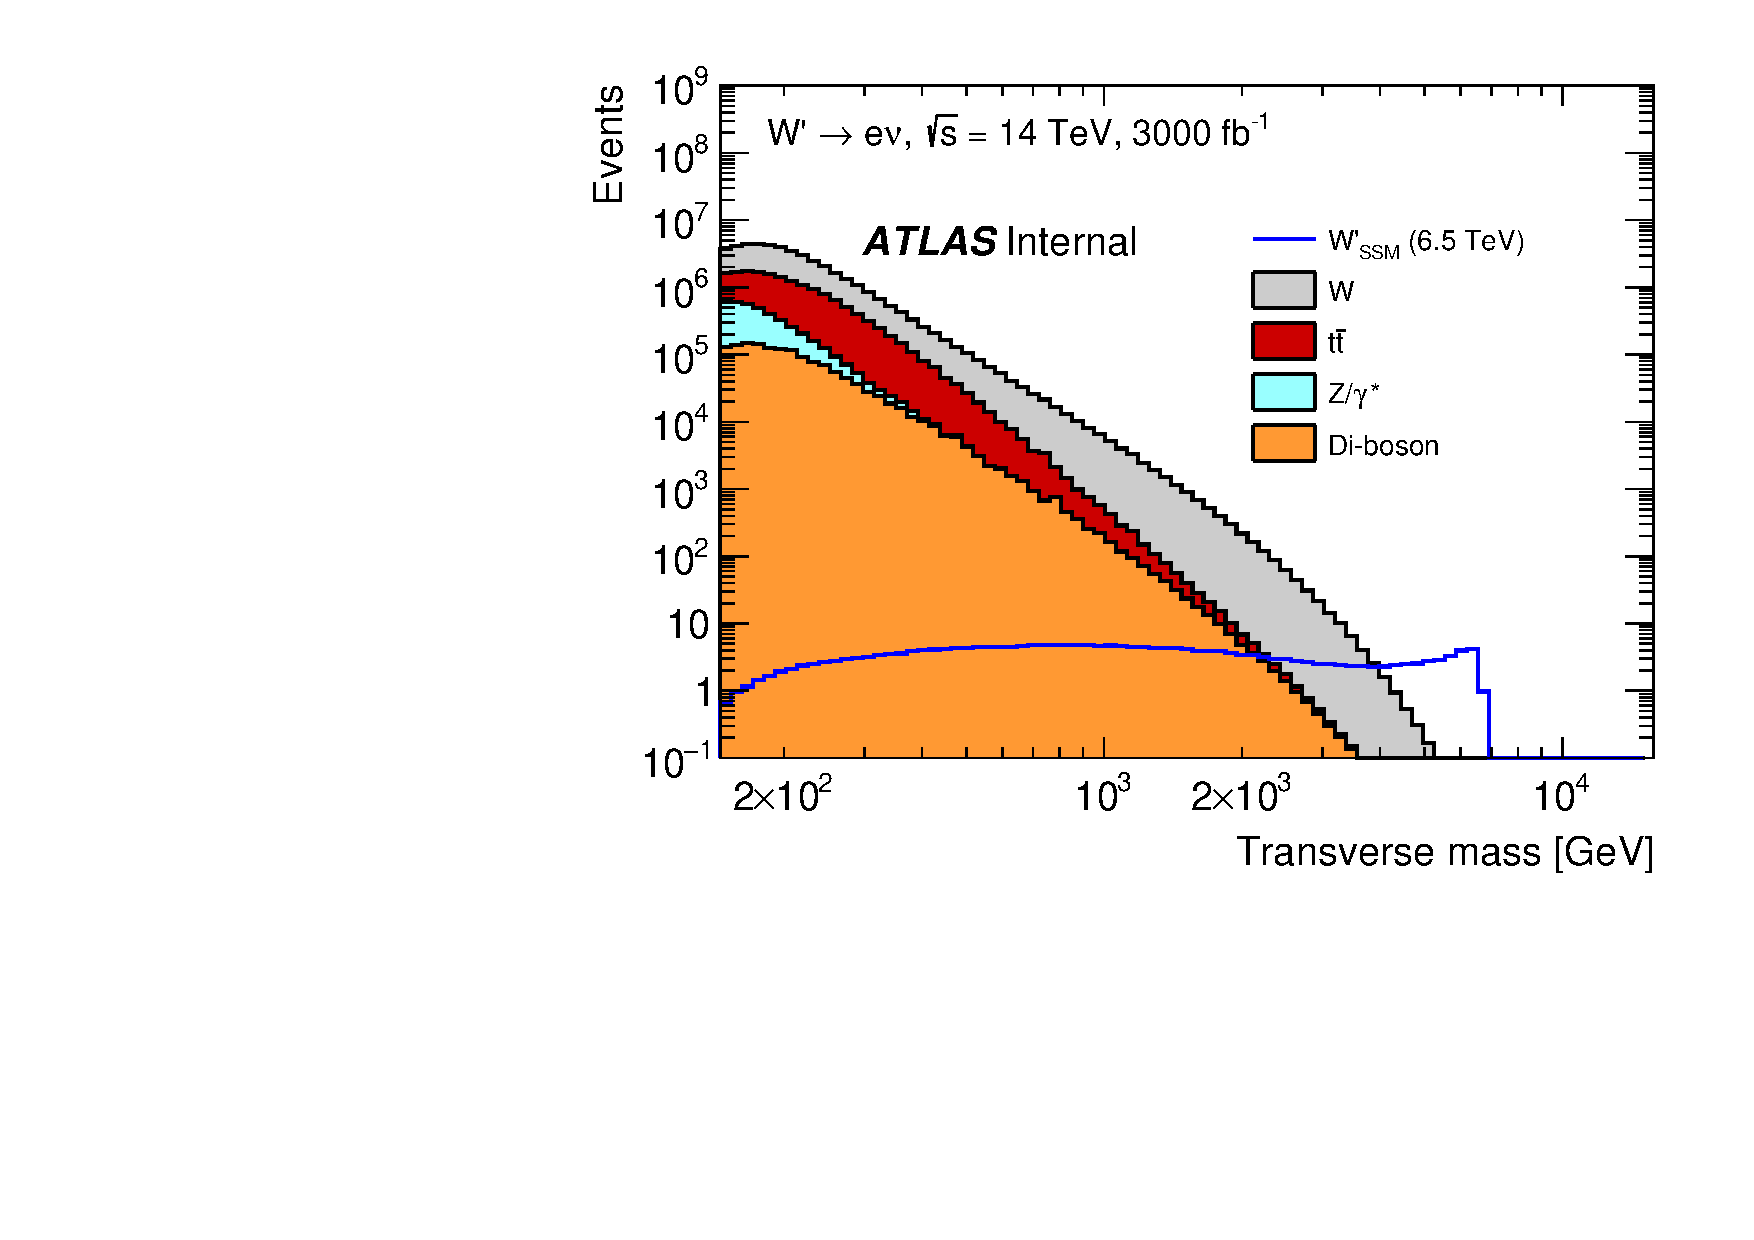
\includegraphics[width=0.49\columnwidth]{./section7OtherSignatures/img/MT_Wenu_6500M.pdf}
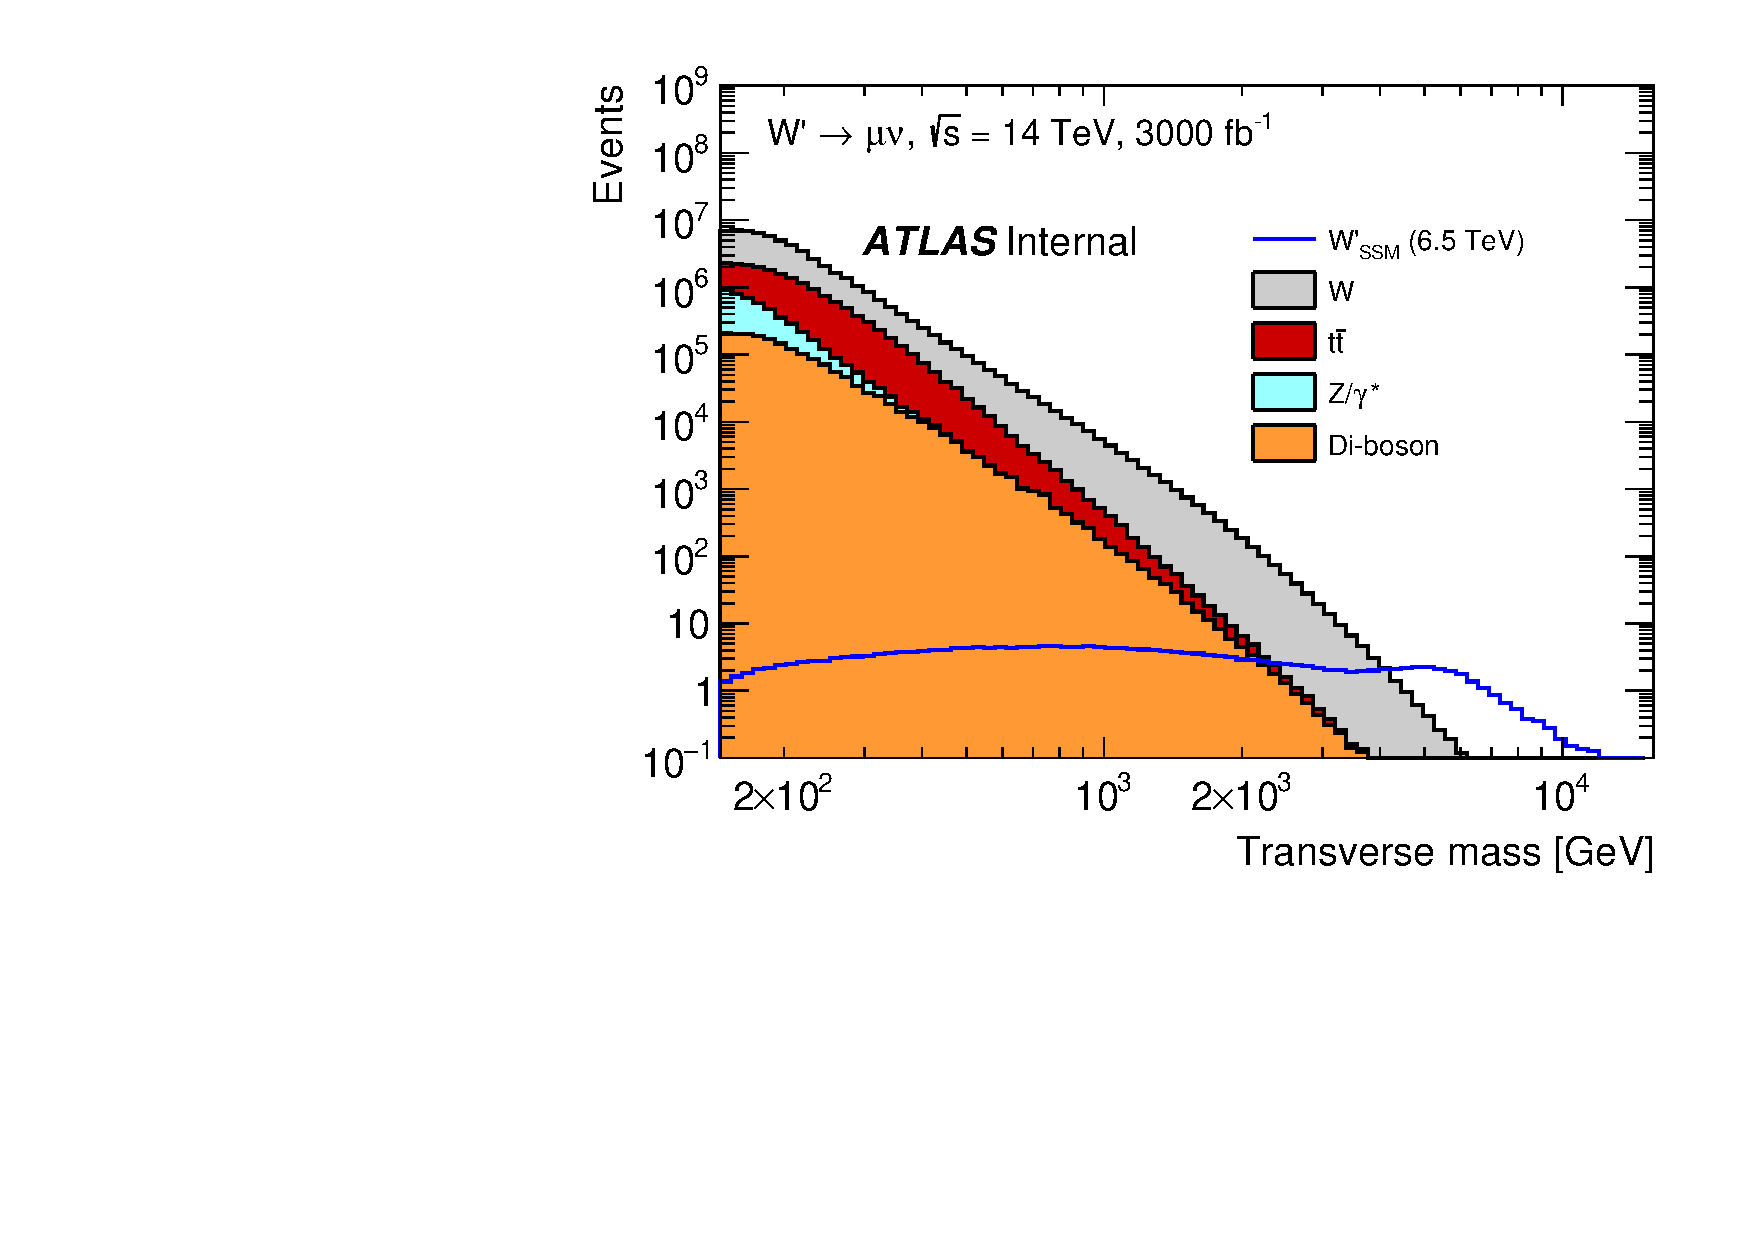
\includegraphics[width=0.49\columnwidth]{./section7OtherSignatures/img/MT_Wmunu_6500M.pdf}
\caption{
  Transverse mass distributions for events satisfying all selection criteria in the electron and muon
  channels of the $W^\prime\to \ell \nu$ search. The different background contributions are shown
  as a stacked sum and the expected signal distributions for a $W^\prime$ boson with a mass of 6.5~TeV
  is shown. The bin width is constant in $\log m_\mathrm{T}$. 
}
  \label{fig:ATLAS_Wprimelv_mT}
\end{figure}

Systematic uncertainties arise from both experimental and theoretical sources.
Since the uncertainties from the Run~2 analysis are found to increase as a function of $m_\mathrm{T}$
these are parameterised as a percentage of the $m_\mathrm{T}$ value expressed in units of TeV.
The uncertainties are then scaled down to account for the increased statistical power at the HL-LHC
according to recommendations in \citeref{atlasperf}.
The experimental systematic uncertainties due to the reconstruction, identification, and isolation of
muons result in a value of $2.5\% \times m_{\mathrm T}$ [TeV], while these uncertainties are negligible
for electrons. 
Systematic uncertainties due to the energy resolution and scale are set to
$2.5\% \times m_{\mathrm T}$ [TeV].
The main systematic uncertainties in the $E_\mathrm{T}^\mathrm{miss}$ calculation and on the jet energy scale are found
to be negligible in Run 2 and are therefore not considered in this analysis.
Theoretical uncertainties are related to the production cross sections estimated from MC simulation.
The effects when propagated to the total background estimate are significant for charged and neutral current DY, and to some extent for top-quark production, but are negligible for diboson production.
No theoretical uncertainties are considered for the $W^\prime$ boson signal in the statistical analysis.
The largest uncertainties arise from the PDF uncertainty in the DY background.
The uncertainties due to the choice of PDF set are taken to be 
$5\% \times m_{\ell\ell}$~[TeV] and the uncertainties in the parameters of the nominal PDF set are assumed
to be $2.5\% \times m_{\ell\ell}$~[TeV]. 
The uncertainty in the multijet background in the electron channel is assumed to be
$2.5\% \times m_{\mathrm T}$ [TeV].
Overall these uncertainties in the background event yield add up to $\sim 7\% \times m_\mathrm{T}$~[TeV].
As the search looks for an excess in the high $m_\mathrm{T}$ tail, the sensitivity is primarily
limited by the statistical uncertainties.

The statistical analysis relies on a Bayesian approach to set cross section times branching fraction
upper limits and a profile likelihood approach to derive the discovery reach as
for the $Z^\prime \to \ell\ell$ search described above. The branching fraction corresponds to that
for decays into a single lepton generation, assumed to be universal in the combination of the two channels.
The 95\%~\cl upper limit on $\sigma\times\cal{B}$ as a function of $W^\prime$ mass is shown
in \fig{fig:ATLAS_wplnulimits} for an integrated luminosity of 3000~fb$^{-1}$ after
combination of the electron and muon channels.
The upper limits on $\sigma\times\cal{B}$ for $W^\prime$ bosons start to weaken above a pole mass
of $\sim 5$~TeV, which is mainly caused by the combined effect of a rapidly falling signal cross section
towards the kinematic limit and the increasing proportion of the signal being produced off-shell\rt{My usual concern. When the W' starts getting a large off-shell contribution to its production CS, then the bound is not anymore on $\sigma\times\cal{B}$. The bound is on $\sigma(pp\to l\nu)$. A limit on $\sigma\times\cal{B}$ cannot grow at high masses, it should be constant.} in
the low-$m_\mathrm{T}$ tail of the signal distribution.
The $W^\prime$ bosons in the SSM can be excluded up to masses of 7.6 (7.3)~TeV in the electron (muon) channel.
The limits in the electron channel are stronger due to the superior energy resolution of the calorimeter
for high-momentum electrons as compared to that of the muon spectrometer for high-momentum muons.
The combination of the two channels increases the limits to just over 7.9~TeV. This is an improvement
of more than 2~TeV with respect to the current exclusion limits using 79.8~fb$^{-1}$ of $\sqrt{s}=13$~TeV data.
For comparison, assuming the performance of the upgraded ATLAS detector and a luminosity of 300~fb$^{-1}$,
$W^\prime$ masses up to 6.7~TeV can be excluded for the combined electron and muon channels. Though the detector resolution for the upgraded detector at the HL-LHC are applied, this is a good approximation of the reach with the current detector at the end of LHC Run~3. 
%
\begin{figure}[tpb]
\centering
%\subfigure[]{\includegraphics[width=0.48\columnwidth]{figures/Limit_xsec_wprime_ee_Sys_3000ifb_14TeV.eps} }
%\subfigure[]{\includegraphics[width=0.48\columnwidth]{figures/Limit_xsec_wprime_mm_Sys_3000ifb_14TeV.eps} }
 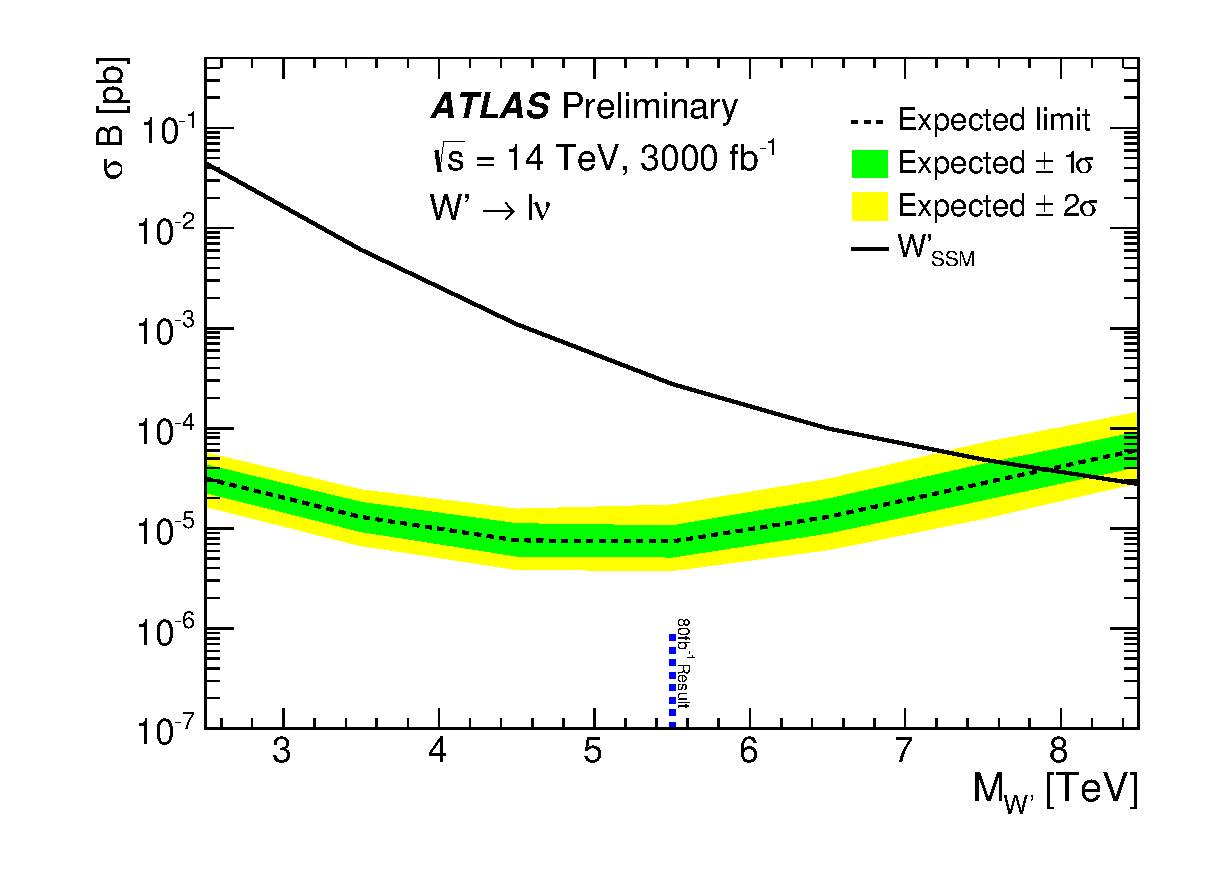
\includegraphics[width=0.48\columnwidth]{./section7OtherSignatures/img/Limit_xsec_wprime_comb_Sys_3000ifb_14TeV.eps}
  \caption{
    Expected (dashed black line) upper limit on cross section times branching fraction ($\sigma\times\cal{B}$)
    as a function of the $W^\prime$ boson mass in the electron, muon, and combined electron and muon channels
    of the $W^\prime \to \ell \nu$ search assuming 3000~fb$^{-1}$ of data. The $1\sigma$ (green) and $2\sigma$
    (yellow) expected limit bands are also shown.
    The predicted $\sigma\times\cal{B}$ for $W^\prime$ production in the SSM is shown as a black line.
    The blue marker shows the current limits obtained with the latest Run~2 analysis based on 79.8~fb$^{-1}$
    of data.
}
  \label{fig:ATLAS_wplnulimits}
\end{figure}
%

The discovery reach is based on a 5-$\sigma$ significance. In the context of the SSM, $W^\prime$ bosons
can be discovered up to masses of 7.7~TeV. The discovery reach is shown in \tabb{tab:ATLAS_wplnulimits}
together with the exclusion limits discussed above.
As can be seen, the discovery reach typically is only few hundred GeV lower than the mass limits obtained
with a background-only hypothesis.
The similarity of the values for the discovery reach and the exclusion limit is expected,
as in the high-$m_\mathrm{T}$ tail the background contribution approaches zero,
while the number of signal events is about three.
The expected reach with 300~fb$^{-1}$ of data will be 1.2~TeV lower assuming the same detector performance. 
\begin{table}[tbp]
  \caption{Expected 95\%~\cl lower limit on the $W^\prime$ mass in the electron and muon channels
    as well as their combination in the context of the SSM assuming 3000~fb$^{-1}$ of data.
    In addition, the discovery reach for finding such new heavy particles is shown.}
  \centering
  \begin{tabular}{c|cc}
    \hline
    \hline
    Decay     &  Exclusion [TeV]& Discovery [TeV]\\
    \hline
    $W^\prime_\mathrm{SSM} \to e\nu$   & 7.6 & 7.5\\
    $W^\prime_\mathrm{SSM} \to \mu\nu$ & 7.3 & 7.1\\ \hline
    $W^\prime_\mathrm{SSM} \to \ell\nu$  & 7.9 & 7.7\\
    \hline
    \hline
  \end{tabular}
  \label{tab:ATLAS_wplnulimits}
\end{table}



\paragraph*{Resonances decaying into a top quark and a bottom quark}

The search for $W^\prime$ bosons in the lepton plus neutrino channel is sensitive to large
mass scales but it is not sensitive to right-handed $W^\prime$ bosons.
This can be alleviated by searching for $W^\prime_{\mathrm{R}} \to t\,\bar{b}$ decays
with subsequent decays $t \to W b$ and $W \to \ell \nu$. 
The final-state signature consists of two $b$-quarks, one charged lepton (electron or muon) and 
$E_{\mathrm{T}}^{\mathrm{miss}}$ from the escaping neutrino. 

Events are required to pass one of the single-lepton triggers: at least one electron
with $p_\mathrm{T} > 22$~GeV and $|\eta|<2.5$ or
at least one muon with $p_\mathrm{T} > 20$~GeV and $|\eta|<2.65$. 
Electrons must satisfy the \textit{tight} identification requirements~\cite{PERF-2013-03} 
requirements and have $p_\mathrm{T} > 25$~GeV and $|\eta| < 2.47$ but outside the barrel--endcap
transition region, $1.37 < |\eta| < 1.52$.
Similarly, muon candidates must meet the \textit{tight} identification criteria~\cite{PERF-2015-10} 
and have $p_\mathrm{T} >25$~GeV and $|\eta| <2.65$. 

The projection study relies on MC simulation for the $W^\prime$ signal
based on \MGvATNLO  with the \textsc{NNPDF23LO} PDF set interfaced to \pythia8 and the A14 tune for the parton shower, hadronisation, and the underlying event. Background for the various top-quark production mechanisms is generated by \powhegbox. In the case of the dominant $t\bar{t}$ background, events are produced withe \textsc{CTEQ6L1} PDF set and interfaced to \pythia6 using the \textsc{Perugia2012} tune~\cite{Skands:2010ak}. $W$+jets events are produced with \MGvATNLO with the \textsc{NNPDF23NLO} PDF set interfaced to \pythia8 and the A14 tune, whereas $Z$+jets events are produced with \powhegbox and the \textsc{CT10} PDF set interfaced to \textsc{Pythia8} and the AU2 tune~\cite{ATL-PHYS-PUB-2012-003}. Diboson events are generated as for the $W^\prime \to \ell\nu$ search above.

The dominant background processes are the production of $t\bar{t}$ pairs and $W+$jets. 
Smaller contributions are also expected from single top quarks ($t$-channel, $Wt$ and $s$-channel), 
$Z+$jets and diboson ($WW$, $WZ$, and $ZZ$) production. 
All background processes are modelled with MC simulation. 
Instrumental background coming from misidentified electrons, referred to as the multijet 
background, is also present but it is very small and further suppressed by applying dedicated 
selection criteria, and it is neglected in the following.
Events are required to satisfy $E_{\mathrm{T}}^{\mathrm{miss}}>80$ (30)~GeV in the electron (muon)
channel as well as $m_{\textrm{T}}^W$ + $E_{\mathrm{T}}^{\mathrm{miss}} > 100$~GeV.

The $W^\prime$ candidates are built from $W$ boson and top-quark candidates.
The $W$ bosons are reconstructed from the lepton--$E_{\mathrm{T}}^{\mathrm{miss}}$ system with
the longitudinal momentum component of the neutrino from the $W$ decay extracted by imposing a
$W$-boson mass constraint.
This $W$ boson candidate is then combined with all selected jets in the event to reconstruct
a top-quark candidate as the $W$+jet combination that has a mass closest to the top-quark mass.
The jet used to form the top-quark candidate is referred to as ``$b_{\mathrm{top}}$''.
Finally, the candidate $W^\prime$ boson is reconstructed by combining the top-quark candidate with
the  highest-$p_{\mathrm{T}}$ remaining jet (referred to as ``$b_1$''). 
The invariant mass of the reconstructed $W^\prime \rightarrow t\bar{b}$ system ($m_{t\bar{b}}$) 
is the discriminating variable of this search. 
An event selection common to all signal regions is defined as: lepton 
$p_{\textrm{T}}>50$~GeV, $p_{\textrm{T}}(b_1)> 200$~GeV, and
$p_{\textrm{T}}({\textrm{top}})> 200$~GeV. As the signal events are expected to be boosted, 
the angular separation between the lepton and $b_{\text{top}}$ is required to satisfy 
$\Delta R(\ell, b_{\text{top}})<1.0$. 

The phase space is divided into eight signal regions (SR) defined by the number of jets and 
$b$-tagged jets, and are labelled as ``$X$-jet $Y$-tag'' where $X=2, 3$ and $Y=1, 2$, 
that are further separated into electron and muon channels.
The signal selection acceptance times efficiency rises from $\sim 4.4\%$ (7.7\%) at
a $W^\prime_{\mathrm{R}}$ mass of 1~TeV to 4.6\% (11.0\%) at 2~TeV, then decreasing to
2.6\% (8.2\%) at 5~TeV in the electron (muon) channel. This decrease is due to the
$b$-tagging performance and the higher boost at higher mass.
The muon channel outperforms the electron channel due to overlap removal requirements, 
as they are relaxed by using a variable $\Delta R$ cone size. The variable $\Delta R$ cone size is not used 
for electrons because of the possible double counting of the energies of electron and jet.

Systematic uncertainties are evaluated following the analysis of 36.1~fb$^{-1}$ of
$\sqrt{s}=13$~TeV $pp$ data in~\citeref{Aaboud:2018jux}
and then scaled according to the recommendations in \citeref{atlasperf}. 
The uncertainty in the luminosity (1\%) and in the theory cross sections (5\% for diboson, 10\% for 
$Z+$jets, and 3\% for single top) are included in the expected limits 
and significance calculation. The $b$-tagging and the modelling uncertainties (which are the dominant 
uncertainties in the shape of the discriminating variable from the previous analysis) are also included.

The presence of a massive resonance is tested by simultaneously fitting the $m_{tb}$
templates of the signal and background simulated event samples using a binned 
maximum--likelihood approach (ML).
%based on the \textsc{RooStats} framework~\cite{Moneta:1289965,Verkerke:2003ir,Baak:2014wma}.
Each signal region is 
treated as an independent search channel with correlated systematic uncertainties.

The normalisations of the $t\bar{t}$ and $W+$jets backgrounds were found to be different than one 
in the analysis of 36.1~fb$^{-1}$, therefore they are free parameters in the fit. They are 
constrained by Asimov dataset to one by construction. 
The other background normalisations are assigned Gaussian priors based on their 
respective normalisation uncertainties. 
The signal normalisation is a free parameter in the fit.

As an example, the $m_{tb}$ distributions for two of the eight signal regions after the ML fit are shown
in \fig{fig:SRmtb2jet} for the expected background and signal contribution corresponding to a
$W^\prime_{\mathrm{R}}$ boson with a mass of 3~TeV.
The binning of the $m_{tb}$ distribution is chosen to optimise the search sensitivity while minimising statistical fluctuations. 
%Requirements are imposed on the expected number of background events per bin, and the bin width is adapted to a resolution function that represents the 
%width of the reconstructed mass peak for each studied \WpR\ boson signal sample. This results 
%in different number of bins in each region.

\begin{figure}[t]
\centering
%\includegraphics[width=0.40\textwidth]{figures/Wptb_2jets_1tag_el_14TeV.pdf}
%\includegraphics[width=0.40\textwidth]{figures/Wptb_2jets_1tag_mu_14TeV.pdf}\\
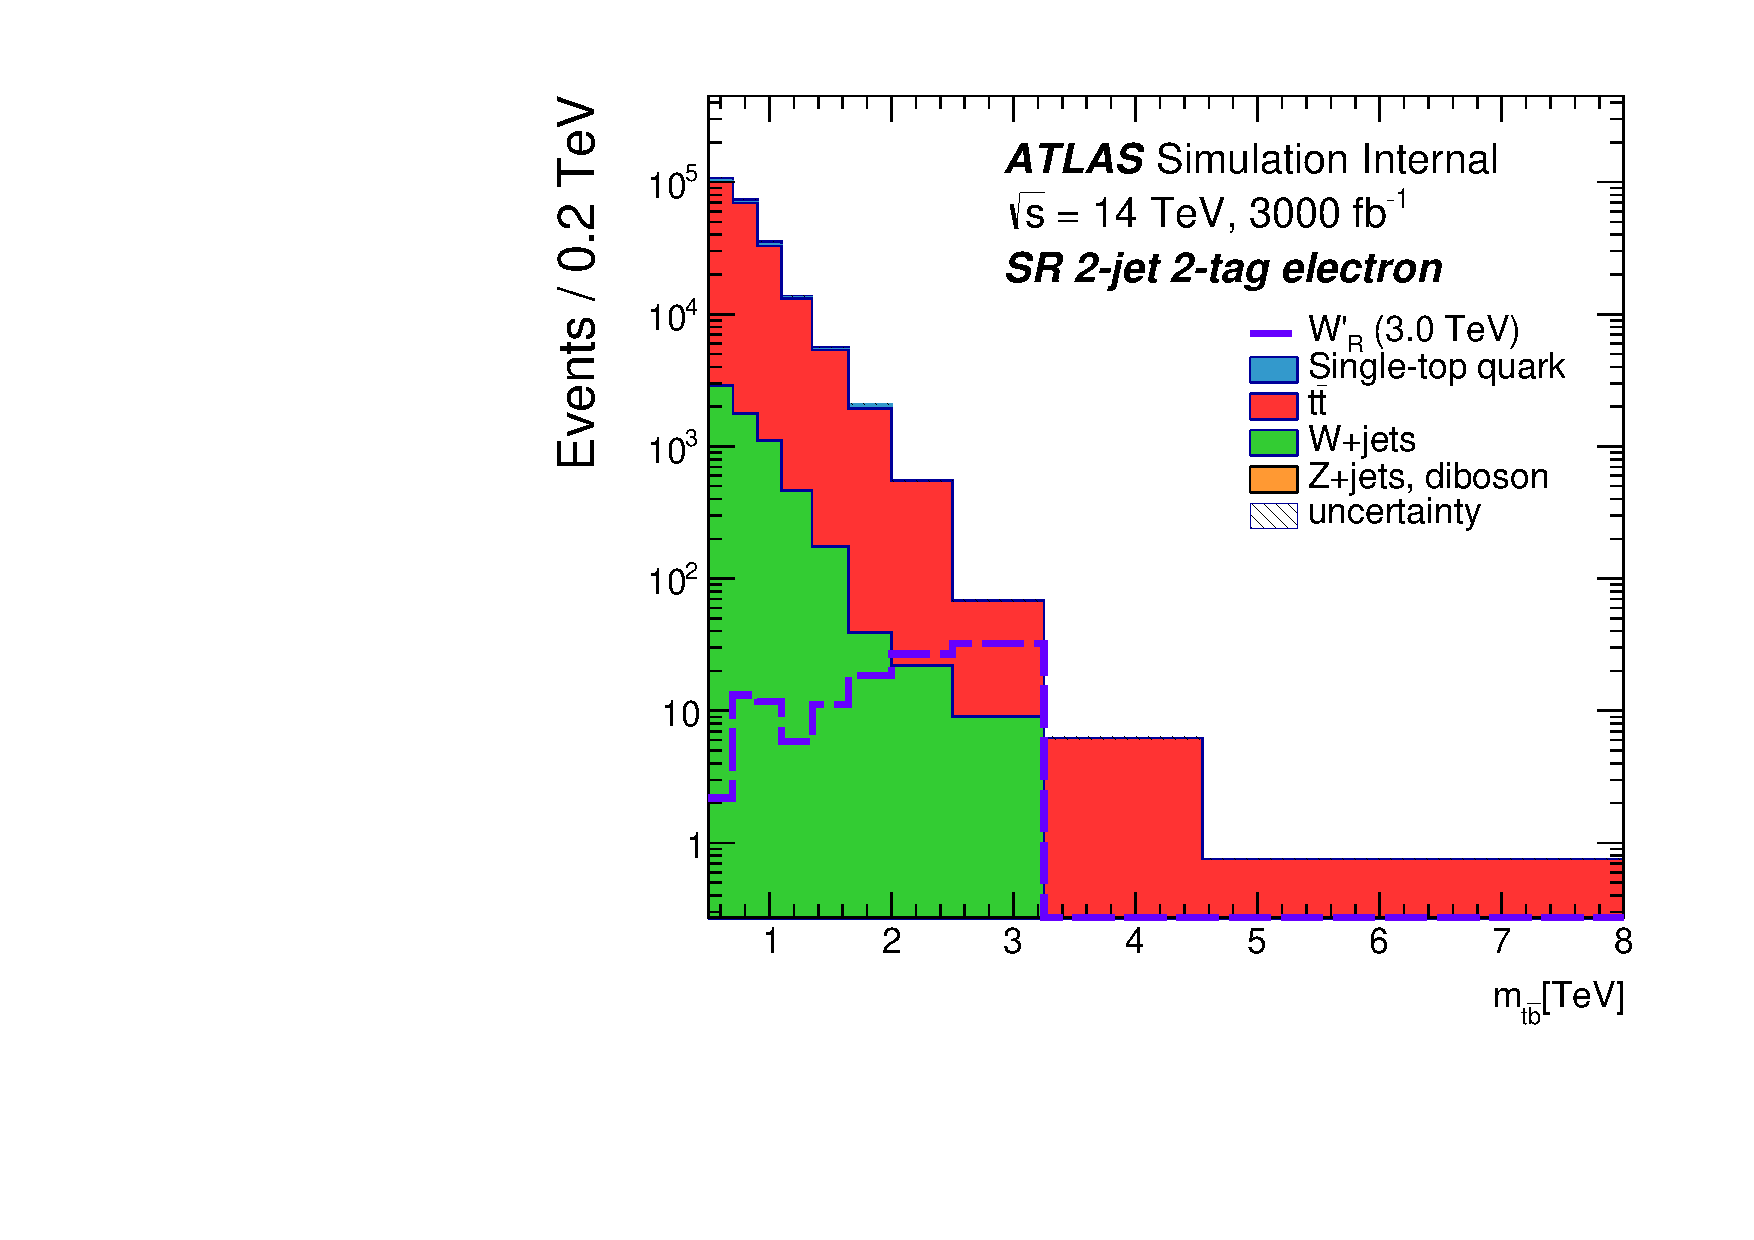
\includegraphics[width=0.48\textwidth]{./section7OtherSignatures/img/Wptb_2jets_2tag_el_14TeV.pdf}
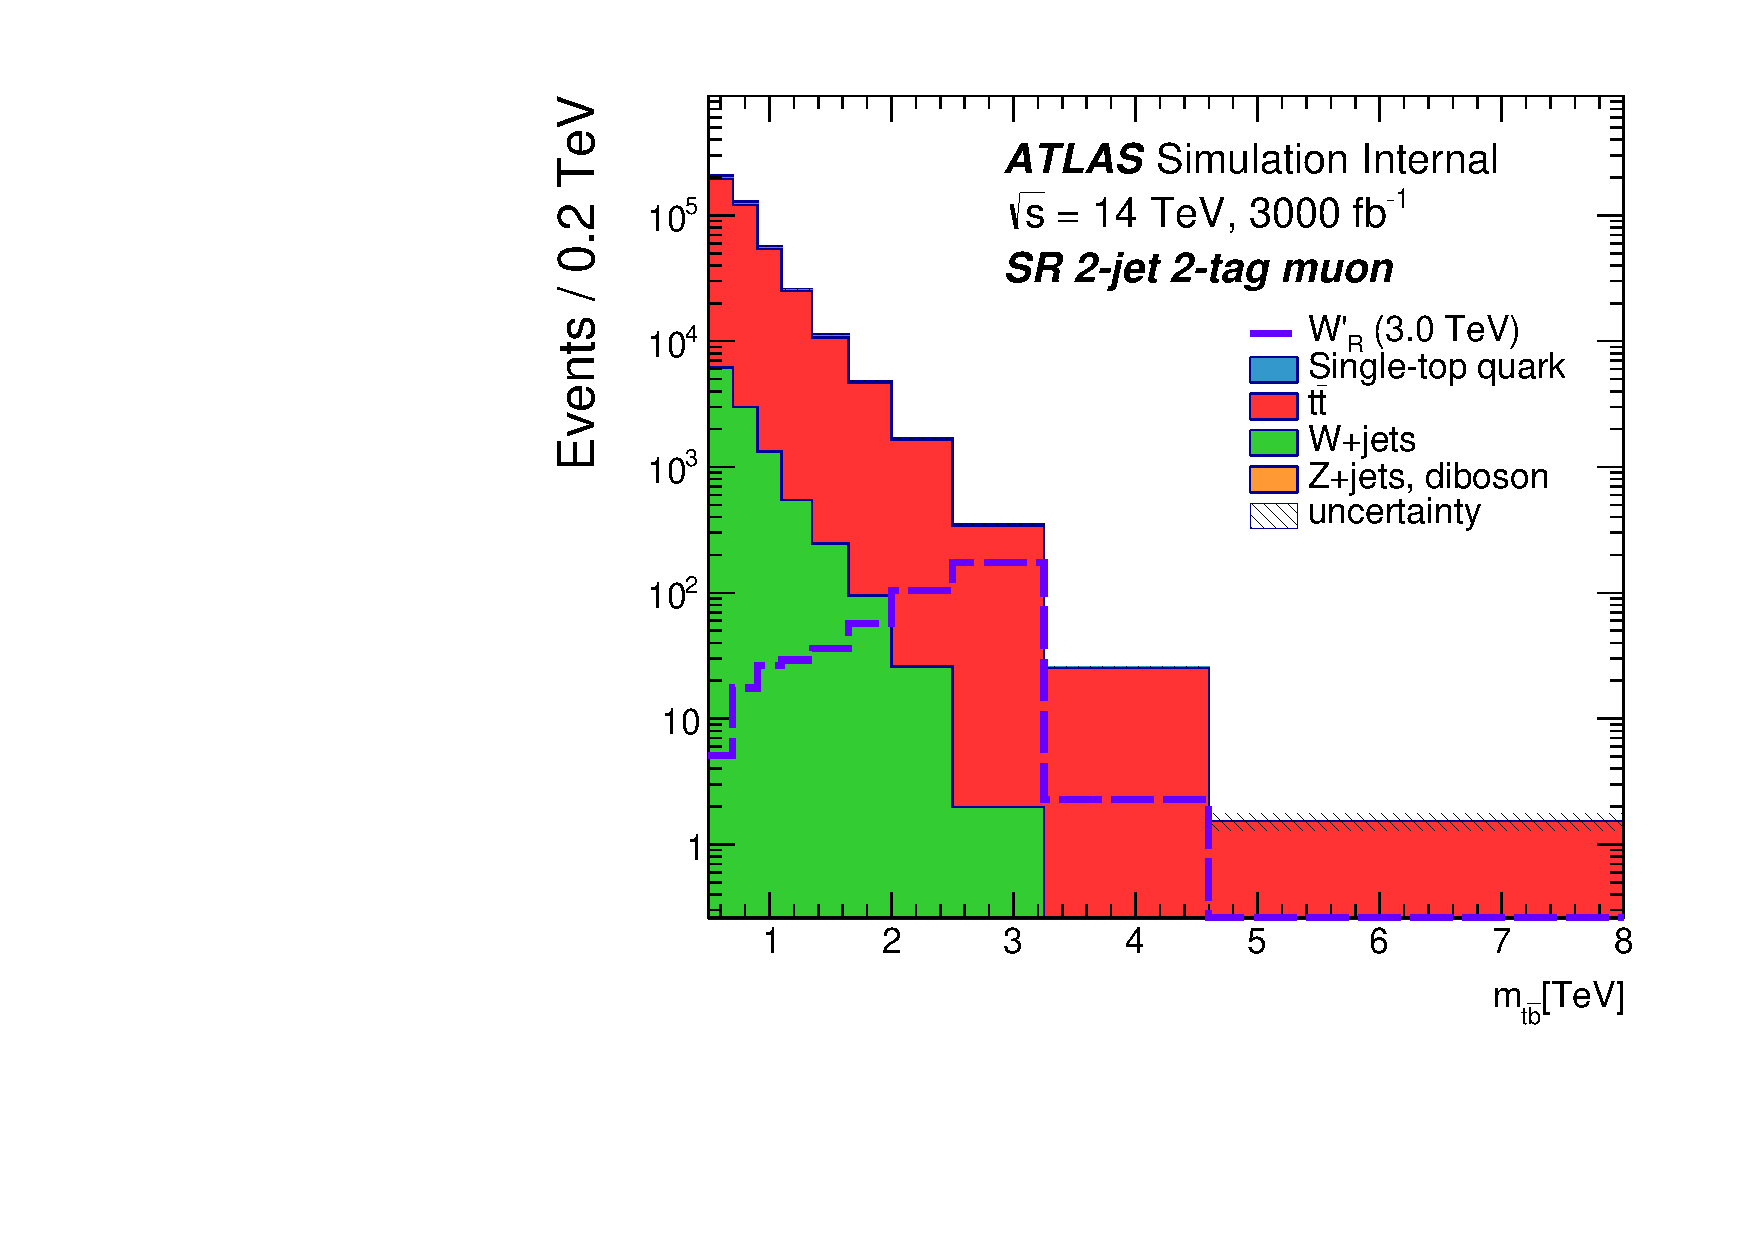
\includegraphics[width=0.48\textwidth]{./section7OtherSignatures/img/Wptb_2jets_2tag_mu_14TeV.pdf}
\caption{Post-fit distributions of the reconstructed mass of the $W^\prime_{\mathrm{R}}$ boson candidate
  in the 2-jet 2-tag signal region for the electron (left) and muon (right) channels. 
  An expected signal contribution corresponding to a $W^\prime_{\mathrm{R}}$ boson mass of 3~TeV is shown.
  Uncertainty bands include all systematic uncertainties.}
\label{fig:SRmtb2jet}
\end{figure}

The limits are evaluated assuming the modified frequentist CL$_\text{s}$ method~\cite{Read:2002hq}
with a \sloppy\mbox{profile-likelihood-ratio} test statistic~\cite{Cowan:2010js} and using the asymptotic approximation. 
The 95\%~\cl upper limits on the production cross section multiplied by the 
branching fraction for $W^\prime_{\mathrm{R}} \rightarrow t\bar{b}$ are shown in \fig{fig:ATLAS_wpLimit}
as a function of the resonance mass for 3000~fb$^{-1}$.
The expected exclusion limits range between $0.02$~pb and $6\times 10^{-3}$~pb for
$W^\prime_{\mathrm{R}}$ boson masses from 1~TeV to 7~TeV.
The existence of $W^\prime_{\mathrm{R}}$ bosons with masses below 4.9~TeV is expected to be excluded,
assuming that the $W^\prime_{\mathrm{R}}$ coupling $g^\prime$ is equal to the SM weak coupling constant $g$. 
This would increase the limit obtained with 36.1 fb$^{-1}$~\cite{Aaboud:2018jux} by 1.8~TeV.

\begin{figure}[t]
  \centering
  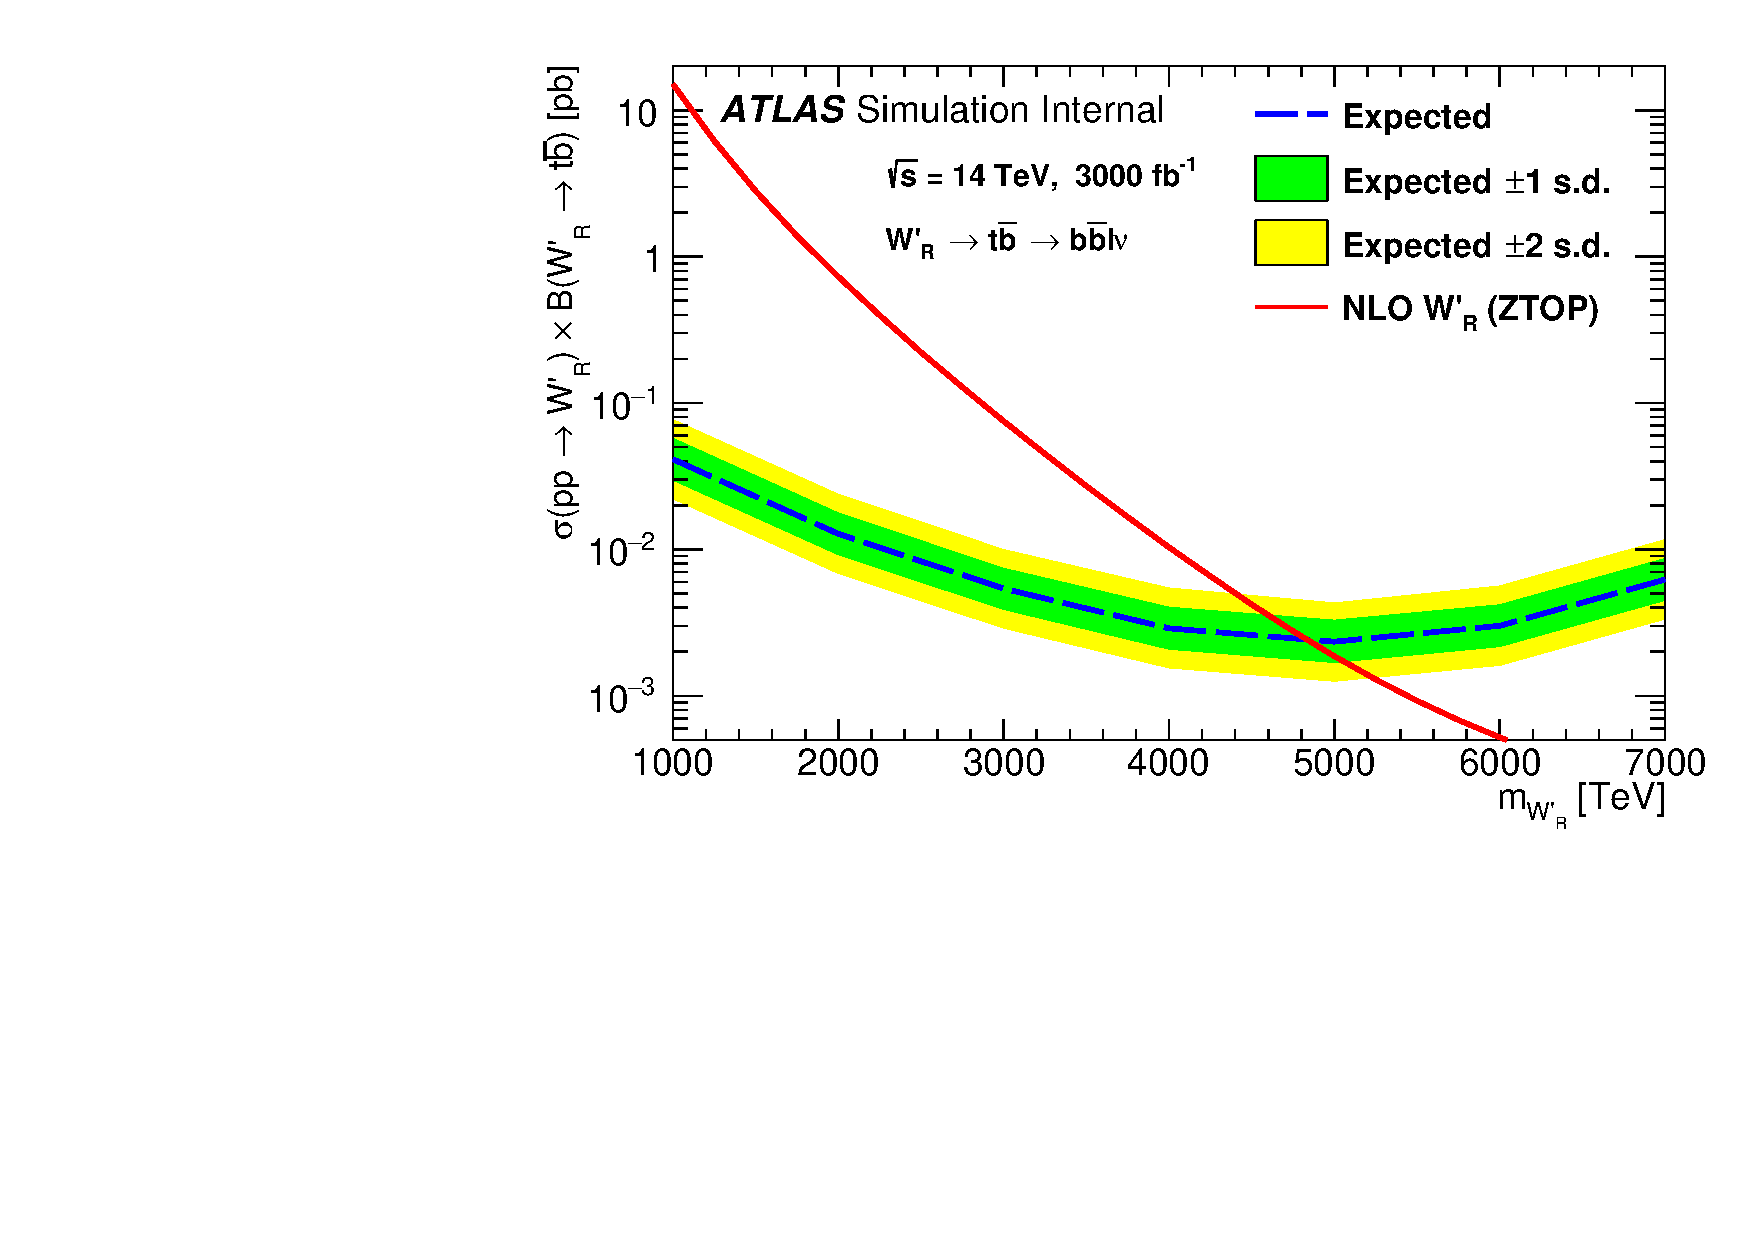
\includegraphics[width=0.55\textwidth]{./section7OtherSignatures/img/Wptb_expected_limit_14TeV.pdf}
  \caption{Upper limits at the 95\%~\cl on the $W^\prime_{\mathrm{R}}$ production cross section times
    branching fraction as a function of resonance mass. The dashed curve and shaded bands correspond
    to the limit expected in the absence of signal and the regions enclosing one/two standard deviation
    (s.d.) fluctuations of the expected limit. The theory prediction is also shown. 
}
\label{fig:ATLAS_wpLimit}
\end{figure}

The expected discovery significance is calculated using the profile likelihood test statistic for
different mass hypotheses for a luminosity of 3000~fb$^{-1}$ with the asymptotic approximation.
Based on 5$\sigma$ significance, it is found that $W^\prime_{\mathrm{R}}$ with masses up to 4.3~TeV
can be discovered at the HL-LHC.

